\chapter{Design and Specification}\label{ch_method}

\section{Aim/vision}

The idea of the game is to travel around the world without physically
having to be there, inviting the user to realise the scale of the
world whilst gaining the positive benefits of outdoor exercise. A user
may decide to run around areas in Scotland (the Scotland Mission) and
this is achieved through routes such as Glasgow to Edinburgh. Each
route is further broken up into manageable stages of a few kilometres
and users are awarded badges based on stages/routes completed and
overall distance and time. Therefore the user can gain short-term
success while working towards the satisfaction of larger goals. 

This approach is to examine whether or not this type of encouragement
could potentially work with outdoor exercise. Metrics will be tracked
for individual users to monitor their exercise duration and frequency
and will be used to encourage that user to exercise. These metics will
then be used to form the basis of our conclusion.

The aims of the project are then as follows:

\begin{enumerate}
  \item To provide incentives that become intrinsically
    rewarding. Rewards are primarily linked to stage and route 
    completion and these accumulate to the completion of the entire
    mission - every achievement brings the user closer to a larger
    success. 
  \item To provide long and short term goals to fulfil the sense of
    achievement. The long term goals are Route completion and these are
    fulfilled by the easily achievable short term goals of Stages -
    for example the Central Park Route contains four stages, one for
    each edge of the park and these stages are easily achievable in an
    exercise session.
    \begin{enumerate}
      \item Stage completion - unlock a photograph of the stage or of
        a key landmark near the stage. This is achieved by completing
        a specific stage.
      \item Route Completion - a gold, silver or bronze medal is
        awarded for completing a route in a given time period. A route
        is completed when all the stages in a route are completed.
    \end{enumerate}
\end{enumerate}


\section{Specification}
\label{sec:specification}
The implementation specifics of this project are defined herein with
the overall development of the project shown in the following sections.

An overarching goal for this implementation is to minimise the end cost
for the user. This cost takes two forms: response time for data
loading and network costs incurred through data loading.

Initial response time for loading data cannot be avoided without
prepackaging content inside the app. We do not want the user to be
forced to update the app every time we want to add another route to
run down so prepackaging will not work. We can however cache the data
we know does not change and reference that instead - which is much
faster than a network response time.

Caching also reduces the overall network cost: by caching the data
received we remove the need to make the request again. This inherently
reduces the network cost by reducing the number of network requests.

These are discussed in more detail in Section \ref{sec:notable} and
will be referenced in the following subsections.

\subsection{Platform and Frameworks}
The mobile application is developed using PhoneGap \cite{phonegap}, 
a tool which allows you to develop a mobile app as if it were
a web app, and then package it as a mobile app. The decision to use
PhoneGap instead of building a native app is primarily because I come
from a web development background but also so we can deploy to
multiple platforms easily without needing to change the code base. 

Because of this, our application is written using HTML, JavaScript,
and CSS3. The twitter Bootstrap CSS framework \cite{bootstrap} was
used because of the excellent support for small screen devices and
layout management. 

Titanium, developed by appcelerator\cite{titanium}, is an alternative
platform to PhoneGap that was also considered. This required a greater
knowledge of android than PhoneGap does but the biggest drawback was
the state of development when the project started. After discussion
with members of the startup community who were using Titanium, it was
apparent that Titanium was still a work in progress and probably a
risk to go with. The platform is now flourishing and would probably
have been the better choice to go with in retrospect, but at the
begining of the project the safer choice was to develop for PhoneGap.

AngularJS\cite{angularjs} is the framework used for the
application. This framework has a major benefit of explicit data linking
between the DOM(Document-Object Model) and the javascript controlling
that section of the DOM. In AngularJS, a controller is defined to
manage the behaviour of a specific section of a page. By defining
these controllers, we can utilise this explicit data linking to manage
how information is displayed in the DOM - if a variable changes in a
controller then it also updates in the DOM. This linking is
bi-directional, so the reverse is also true. 

The AngularJS framework also facilitates many other control
mechanisms: DOM tree manipulations, CSS class manipulations, frontend
routing (a process where a section of the DOM tree and an associated
JavaScript controller are swapped out based on the current URL) and
wrappers around the browsers native AJAX implementation. All of this
functionality make AngularJS the ideal framework for the project. 

The web application is written in Python and uses Django\cite{django}
and Django-Tastypie\cite{tastypie}. Django is used as a middleware
platform for interfacing with the database and creation of specific
workflow interactions; while Django-Tastypie is used for managing and
building a REST style API for well-defined database object access.

Django exposes an Object-Relation Mapping (ORM) inside the framework
for manipulating and creating database objects. This is utilised by
Django-Tastpie for creation of the REST API. We use a REST style API
so that the mobile app is able to uniquely identify an object in the
database in a consistent and reliable manner. This is used in 
session management in Section \ref{sec:session_mgmt}.

Moreover, there is a large number of database objects that we require
knowledge about in the app. A tool which creates a well defined way of
accessing these objects and managing their access permissions is
invaluable for consistency and reliability.

No session-like state is required in this application as the database
object relations are defined in such a way that they hold all
information required. 

\subsection{N-Tier Diagram}
The high level components of this system are reasonably simple (figure
\ref{NTier}). The
user requires a mobile phone with GPS enabled, an active internet
connection and the mobile application installed. This communicates
with a Django Webserver with a REST-style API (with a small number of
bespoke views since some behaviour does not fit well with the REST
specification) which in turn uses Django's Object Relation Model (ORM)
to persist these to a database.

The mobile application communicates with the devices GPS location
management system to obtain location information for the
user. We request that the users devices provides us with the most
accurate GPS location it can provide, so it will try satellite
positioning first and then try network provided information.
\begin{figure}[H]
  \centering
  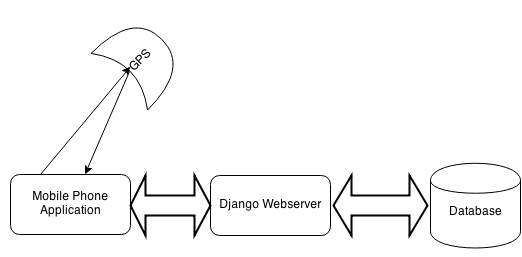
\includegraphics[width=\textwidth]{images/N-tier.png}
  \caption{N-Tier diagram}
  \label{NTier}
\end{figure}

\subsection{Entity Relation Diagram}
\label{sec:ER}
There have been two significant iterations of the Entity Relation (ER)
diagram in this project - the first (figure \ref{ER_1}) is the final
theoretical ER model and the second is the real world implementation
with modifications and extra linking for data transfer optimisation
and changing requirements.

The main reason for the implementation modifications is to keep data
transfer low between the mobile device and the API. Since the mobile
device will be using non-wifi based communication methods the number
of bytes transferred will be logged by their network provider and will
cost the end user. Since we care for the monetary cost that using the
app may incur to the end user (Section \ref{sec:consideration}), we can
sacrifice having a non-redundant database in order to optimise the
data transfer for the end user.

\begin{figure}[H]
  \centering
  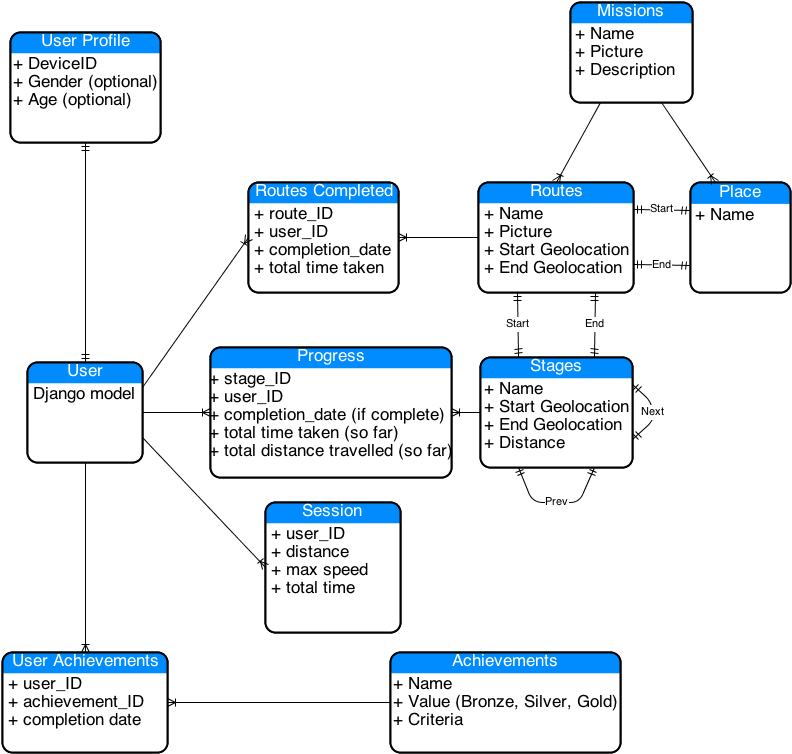
\includegraphics[width=\textwidth]{images/ER.png}
  \caption{ER diagram, final theoretical model}
  \label{ER_1}
\end{figure}

\todo{Do implementation ER diagram}



\subsection{Walkthrough of Wireframes}
\todo{THIS NEEDS REDONE WITH NEW WIREFRAMES}

When the app is launched it silently registers with the server
allowing the user to use the app immediately. The user is then shown
the middle-top screen.
\begin{enumerate}
\item From the middle top screen, the user can follow arrow 1 by
  clicking on the middle button ``Pick Mission'' to pick a Mission
  (Run around Arran or Egg for example) and then pick a start and
  end location. After confirming these choices, the user is taken
  back to the middle top screen, or at any time can click the
  ``Home'' button to return. 
\item The user can also view their current acheivements by clicking
  the ``Achievements'' button on the middle top screen, following
  arrow 2. These achievements will be grouped by tabs by category -
  Distance, Time, Stage and Mission based achievements.
\item The user can follow arrow 3 from the middle top screen to
  notify the app that they are starting an exercise period, telling
  the app to track their distance. If a Mission and start and end
  location are not picked (as in point 1) then they will instead be
  redirected to this screen and are unable to start exercising until
  this choice has been made. Once they have successfully advanced to
  this screen, it will display their current progress as they move
  showing the user how close to completion of their current stage
  and overall route they are. 
\item When the user has finished exercising, they will click the
  ``End Session'' button and be taken to the first summary screen -
  following arrow 4. Here statistics from their exercise will be
  shown and the option to share this on several social media
  outlets.
\item The user can then move to the second and final summary screen,
  following arrow 5, where they will be shown any achievements they
  were awarded during that session. The user will also have the
  option to share these on social media outlets. From here, the user
  can click the ``Home'' button and be taken back to the middle top
  screen. 
\end{enumerate}
\begin{figure}[H]
  \centering
  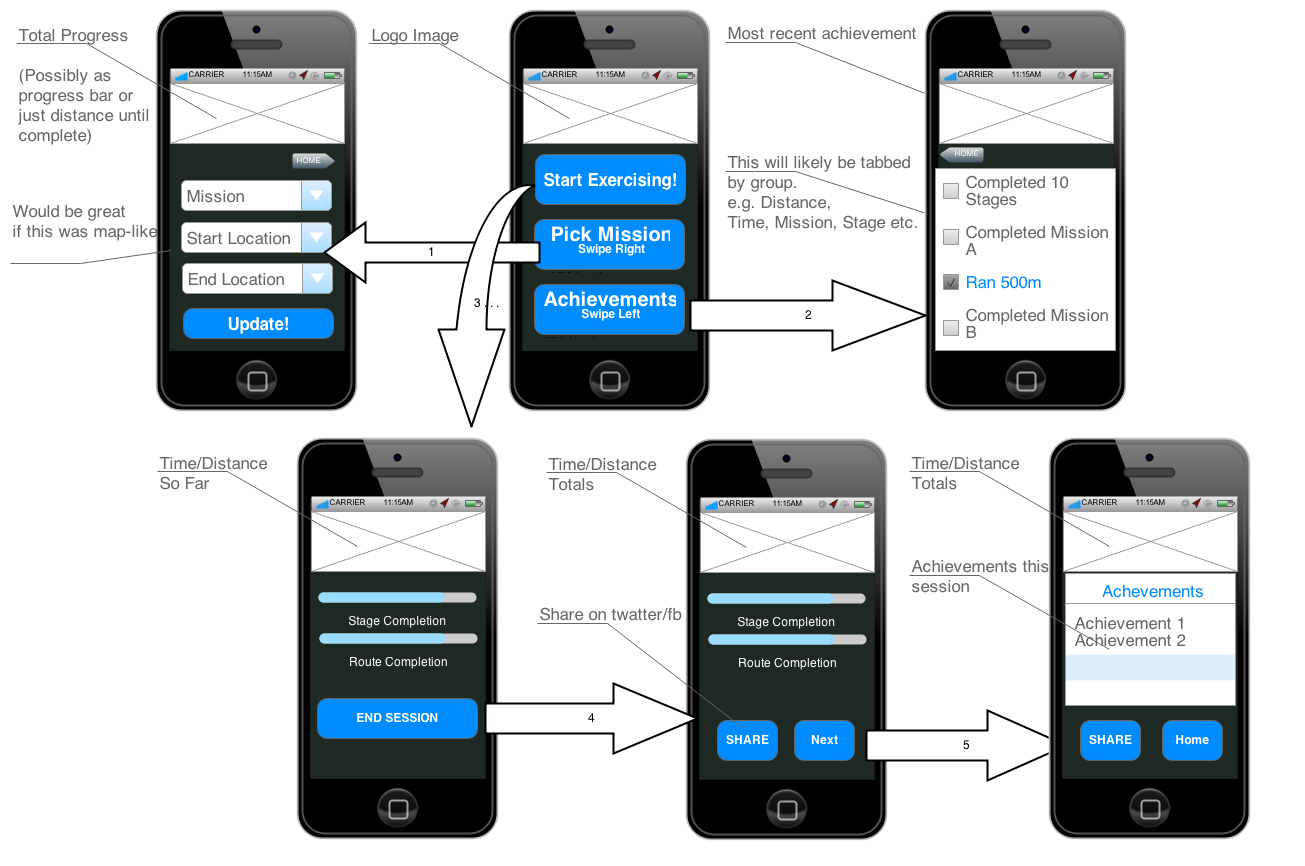
\includegraphics[width=\linewidth]{images/Wireframes.png}
  \caption{Wireframes, initial design}
  \label{wireframes_1}
\end{figure}

\section{Notable design decisions}\label{sec:notable}
\subsection{Explicit caching}
\label{sec:explicit_caching}
As was mentioned in Section \ref{sec:specification}, the minimisation of network
traffic is of great consideration when dealing with mobile devices. We
did not want the mobile device to make repeated API calls for
resources that will not change in the short term - resources such as
what missions are available, what routes belong to what missions and
what stages belong to each route. 

The main case for this is as follows. A user may open the app for the
sole purpose of browsing all missions and their routes, and any
progress they have on these routes before they start using the app for
exercise. In an unmanaged situation the app could call the API each
time it lands on a menu to pick a mission or the routes for a mission
- if the user is browsing then they may see the same information
provided several times. 

If we remove data transfer from the equation all together and focus
solely on the user experience then caching will give a better user
experience in terms of loading speed. Since caching means we do not
have to hit the API each time we want to see something we have seen
before, we can load selection menus faster. 

Note that I only intend to cache data endpoints that are unlikely to
change in the short term or those that cannot feasibly change under
certain circumstances. The ``progress'' endpoint which provides the
data about a users progress along given stages will not change if the
user does not initiate an exercise session - the user has not made any
more progress so it could not have changed. 

These caching services are used as singleton-like facilities in the
application to ensure consistent data throughout the application, an
update to this data will be reflected throughout the entire
application. 

\subsection{Promise Based Module Interfaces}
Each module that has been created for managing either a specific set
of objects(routes, missions or the user object) has been defined
with a common interface. This common interface brings a regular
and well defined way of interacting with these modules, especially if
they utilise explicit caching (section \ref{sec:explicit_caching}) or
execute asynchronous methods.

There are two ways that this consistent interface could be
implemented: a function callback explicitly provided as an argument to
the module function call; or by using promises.

Function callbacks passed as parameters are a common JavaScript
paradigm. They are used in the PhoneGap framework to interface with
the device\cite{phonegap_currentpos}. A frequent problem with function
callbacks is what is colloquially known as ``callback hell''
\cite{callback_hell} where nested anonymous functions are used to
bring an order of execution to asynchronous tasks. This can become
unmanageable and hard to maintain in larger projects but can be
overcome with good software development procedures.

The biggest problem for us is the framework we are using - AngularJS
only knows about events that happen in its own scope. This means that
when we invoke the callback function with the data from a module, the
data will be updated in the controller but AngularJS does not know to
update any reflections of this data in the DOM or elsewhere. There are
ways to notify the framework that it should run an update (known as a
digest cycle)\cite{angularjs_apply} but if we invoke this when a
digest cycle is currently in progress then the framework throws an
error and drops the request.

Another option is to use the AngularJS wrapping for the standard
``setTimeout'' function with a delay of zero. While this may seem
frivolous, a subtlety of this wrapping avoids the digest cycle clash
of the above problem. The AngularJS wrapper ``\$timeout'' will invoke
the function passed to it after the delay expires, but importantly
will cause a natural digest cycle to occur. 


AngularJS\cite{angularjs}, the frontend JavaScript framework, has a 

\subsection{Exercise Session Management}
\label{sec:session_mgmt}
Due to the environmental implications brought on by GPS, a user may
drop out of connection for finding their location. The user should not
be penalised for this as it is outwith their control and is not a
direct error on their part. Something as simple as running through a
tunnel could initiate the loss of signal. 

To counter this, I have designed the exercise session object (herein
referred to as just a ``session'') to accommodate for this.

When a user decides to exercise, a new session is created through the
API. The users device is then given a unique ID for that session that
only they have a knowledge of (in the first iteration of this
implementation this ID is a direct mapping to the ID of the object in
the database, but in a future version this could be something more
obscure). Only this user can update this session and it can only be
updated if you know hte unique ID for that session. 

When you have a GPS location and are ready to update, you know the
unique ID and are able to update the session. If you do not have a GPS
location, then as long as you are still polling for a GPS location the
app will hold onto that unique ID so when you eventually get a GPS
location you can update easily.

The method for updating handles completion of many stages. This
implies that if you update a session and the stage you are currently
exercising on completes you will be immediately moved onto the next
stage on the route, if one is available. This also handles a use case
where you drop out of GPS connection and travel far enough to complete
more than one stage on the route you are on. Then the method will log
your progress on your last known stage, completing it, and then will
complete as many of the next stages as are available and that you have
enough accumulated distance to complete.

When you end the exercise session or close the app, the unique ID for
the session you are on is lost and so cannot be updated. This
effectively ``ends'' the session without explicitly doing so.

This should allow the user to drop in and out of GPS connection
without being penalised for doing so.

\subsection{Distance Verification}

\todo{Need to actually implement this}
